\documentclass[11pt,a4paper]{article}
\usepackage[margin=2.2cm]{geometry}
\usepackage{amsmath,amssymb,booktabs,graphicx,hyperref}
\title{MIS tableaus of \texttt{MultiRate.TimeStepping.mis\_tableau}:\\coefficients and stability on the acoustic-advection test}
\author{MultiRate notes}
\date{\today}
\begin{document}
\sloppy
\maketitle
\noindent\textbf{Convention} (Knoth \& Wensch 2014, ClimaTimeSteppers.jl, Breeze.jl). For $y'=f_{\rm fast}(y)+f_{\rm slow}(y)$,
$Y_0=y^n$, $\Delta Y_j=Y_j-y^n$, stage $i=1,\dots,s$:
\begin{align*}
V(0)&=y^n+\sum_{j<i}\alpha_{ij}\Delta Y_j,\\
V'(\tau)&=f_{\rm fast}(V)+\frac1{d_i}\Big[\sum_{j<i}\gamma_{ij}\frac{\Delta Y_j}{\Delta t}+\sum_{j\le i}\beta_{ij}f_{\rm slow}(Y_{j-1})\Big],\qquad
0\le\tau\le d_i\Delta t,
\end{align*}
$d_i=\sum_j\beta_{ij}$, $Y_i=V(d_i\Delta t)$, $y^{n+1}=Y_s$. $\Sigma d=\sum_id_i$ is the fast integration time per step (in $\Delta t$).
In the notation of \texttt{MISPolynomial.tex}: constant coupling $p_{i+1,j}=\beta_{ij}$, $g_{i+1,j+1}=\gamma_{ij}$,
$\alpha_{i+1,j+1}=\alpha_{ij}$. Stage times $c_i$: the time reached by stage $i$.

\noindent\textbf{Orders} from the bicoloured B-series (\texttt{MultiRate.MIS.order}, residuals $\le10^{-5}$) for the problem
classes: G general $F(y,z)$ (the frozen form), B affine in $z$, A additive $f(y)+g(z)$, L $f(y)+Lz$.

\noindent\textbf{Stability} (Knoth \& Wensch 2014, eq.~(10)): $u_t+Uu_x=-cp_x$, $p_t+Up_x=-cu_x$, periodic C-grid, centred
second-order acoustics (fast), third-order upwind advection (slow), exact fast part; stable region (blue) of
$\max_\theta\rho\le1+10^{-8}$ over $C_{\rm sound}=c\Delta t/\Delta x$ and $C_{\rm adv}=U\Delta t/\Delta x$
(\texttt{examples/mis\_stability\_fv.jl}); orange: the base Runge--Kutta method; dashed: $U/c=1/6$. The computation is
described below.

\subsection*{How the stability plots are computed}
\begin{enumerate}
\item \emph{Symbols.} With $p$ in the cells, $u$ on the faces and the Fourier ansatz $p_k=\hat p\,e^{\mathrm ik\theta}$,
  $u_{k+1/2}=\hat u\,e^{\mathrm i(k+1/2)\theta}$, $\theta\in[0,\pi]$, the semi-discretisation becomes
  $(\hat p,\hat u)'=(C_{\rm adv}S_1(\theta)+C_{\rm sound}L_1(\theta))(\hat p,\hat u)$ per time step $\Delta t=1$, with the
  centred staggered acoustics
  \[
   L_1(\theta)=\begin{pmatrix}0&-(e^{\mathrm i\theta}-1)\\-(1-e^{-\mathrm i\theta})&0\end{pmatrix},\qquad
   \text{eigenvalues }\pm2\mathrm i\sin(\theta/2),
  \]
  and the third-order upwind flux-form advection of both variables,
  $S_1(\theta)=\nu(\theta)I$, $\nu(\theta)=-(2e^{\mathrm i\theta}+3-6e^{-\mathrm i\theta}+e^{-2\mathrm i\theta})/6$
  (\texttt{MultiRate.MIS.fv\_symbols}). The acoustic part is the fast part $L$, the advection the slow part $S$.
\item \emph{MIS step matrix.} Stage $i$ solves $V'=d_iLV+r_i$ on $[0,1]$, $V(0)=I+\sum_j\alpha_{ij}(Y_j-I)$, with the
  constant forcing $r_i=\sum_j\gamma_{ij}(Y_j-I)+\sum_j\beta_{ij}SY_j$; the inner problem is solved exactly (matrix
  exponential of the system augmented by the forcing), i.e.\ the small steps are not part of the analysis. The stage
  recursion gives the $2\times2$ step matrix $R(\theta)$ (\texttt{MultiRate.MIS.amplification}).
\item \emph{Criterion.} A point $(C_{\rm sound},C_{\rm adv})$ is stable if $\max_\theta\rho(R(\theta))\le1+10^{-8}$, with
  40 equidistant $\theta\in[0,\pi]$ (\texttt{max\_amplification}). Grid: $\Delta C_{\rm sound}=0.125$ on $[0,24]$,
  $\Delta C_{\rm adv}=0.05$ on $[0,4]$; blue are the stable grid points, the black line is the level $\rho=1+10^{-8}$.
\item \emph{Base Runge--Kutta method} (orange). The explicit method $(A,b)$ that the MIS method reduces to if $F$ does not
  depend on its second argument (\texttt{base\_method}), applied to the whole operator without fast integration:
  $R=I+b^TZ(I-AZ)^{-1}\mathbf 1$, $Z=C_{\rm adv}S_1+C_{\rm sound}L_1$ (\texttt{rk\_amplification}). At $C_{\rm sound}=0$
  both methods coincide, so the regions agree on the $C_{\rm adv}$ axis; the distance between the orange and the blue
  region in $C_{\rm sound}$ is the gain of the multirate integration.
\item \emph{Line $U/c=1/6$} (dashed), $C_{\rm adv}=C_{\rm sound}/6$: a typical upper bound of the Mach number in the
  atmosphere ($U\approx55$\,m/s, $c\approx340$\,m/s). On this line both Courant numbers grow with $\Delta t$; the value
  ``$U/c=1/6$'' given for each method is the largest $C_{\rm sound}$ (step $1/16$) up to which all points of the line
  are stable, i.e.\ the largest stable time step $\Delta t=C_{\rm sound}\Delta x/c$ at this Mach number.
\item \emph{Tables.} For given $C_{\rm sound}$ the largest $C_{\rm adv}$ such that all smaller $C_{\rm adv}$ are stable
  (from the grid).
\end{enumerate}

\begin{center}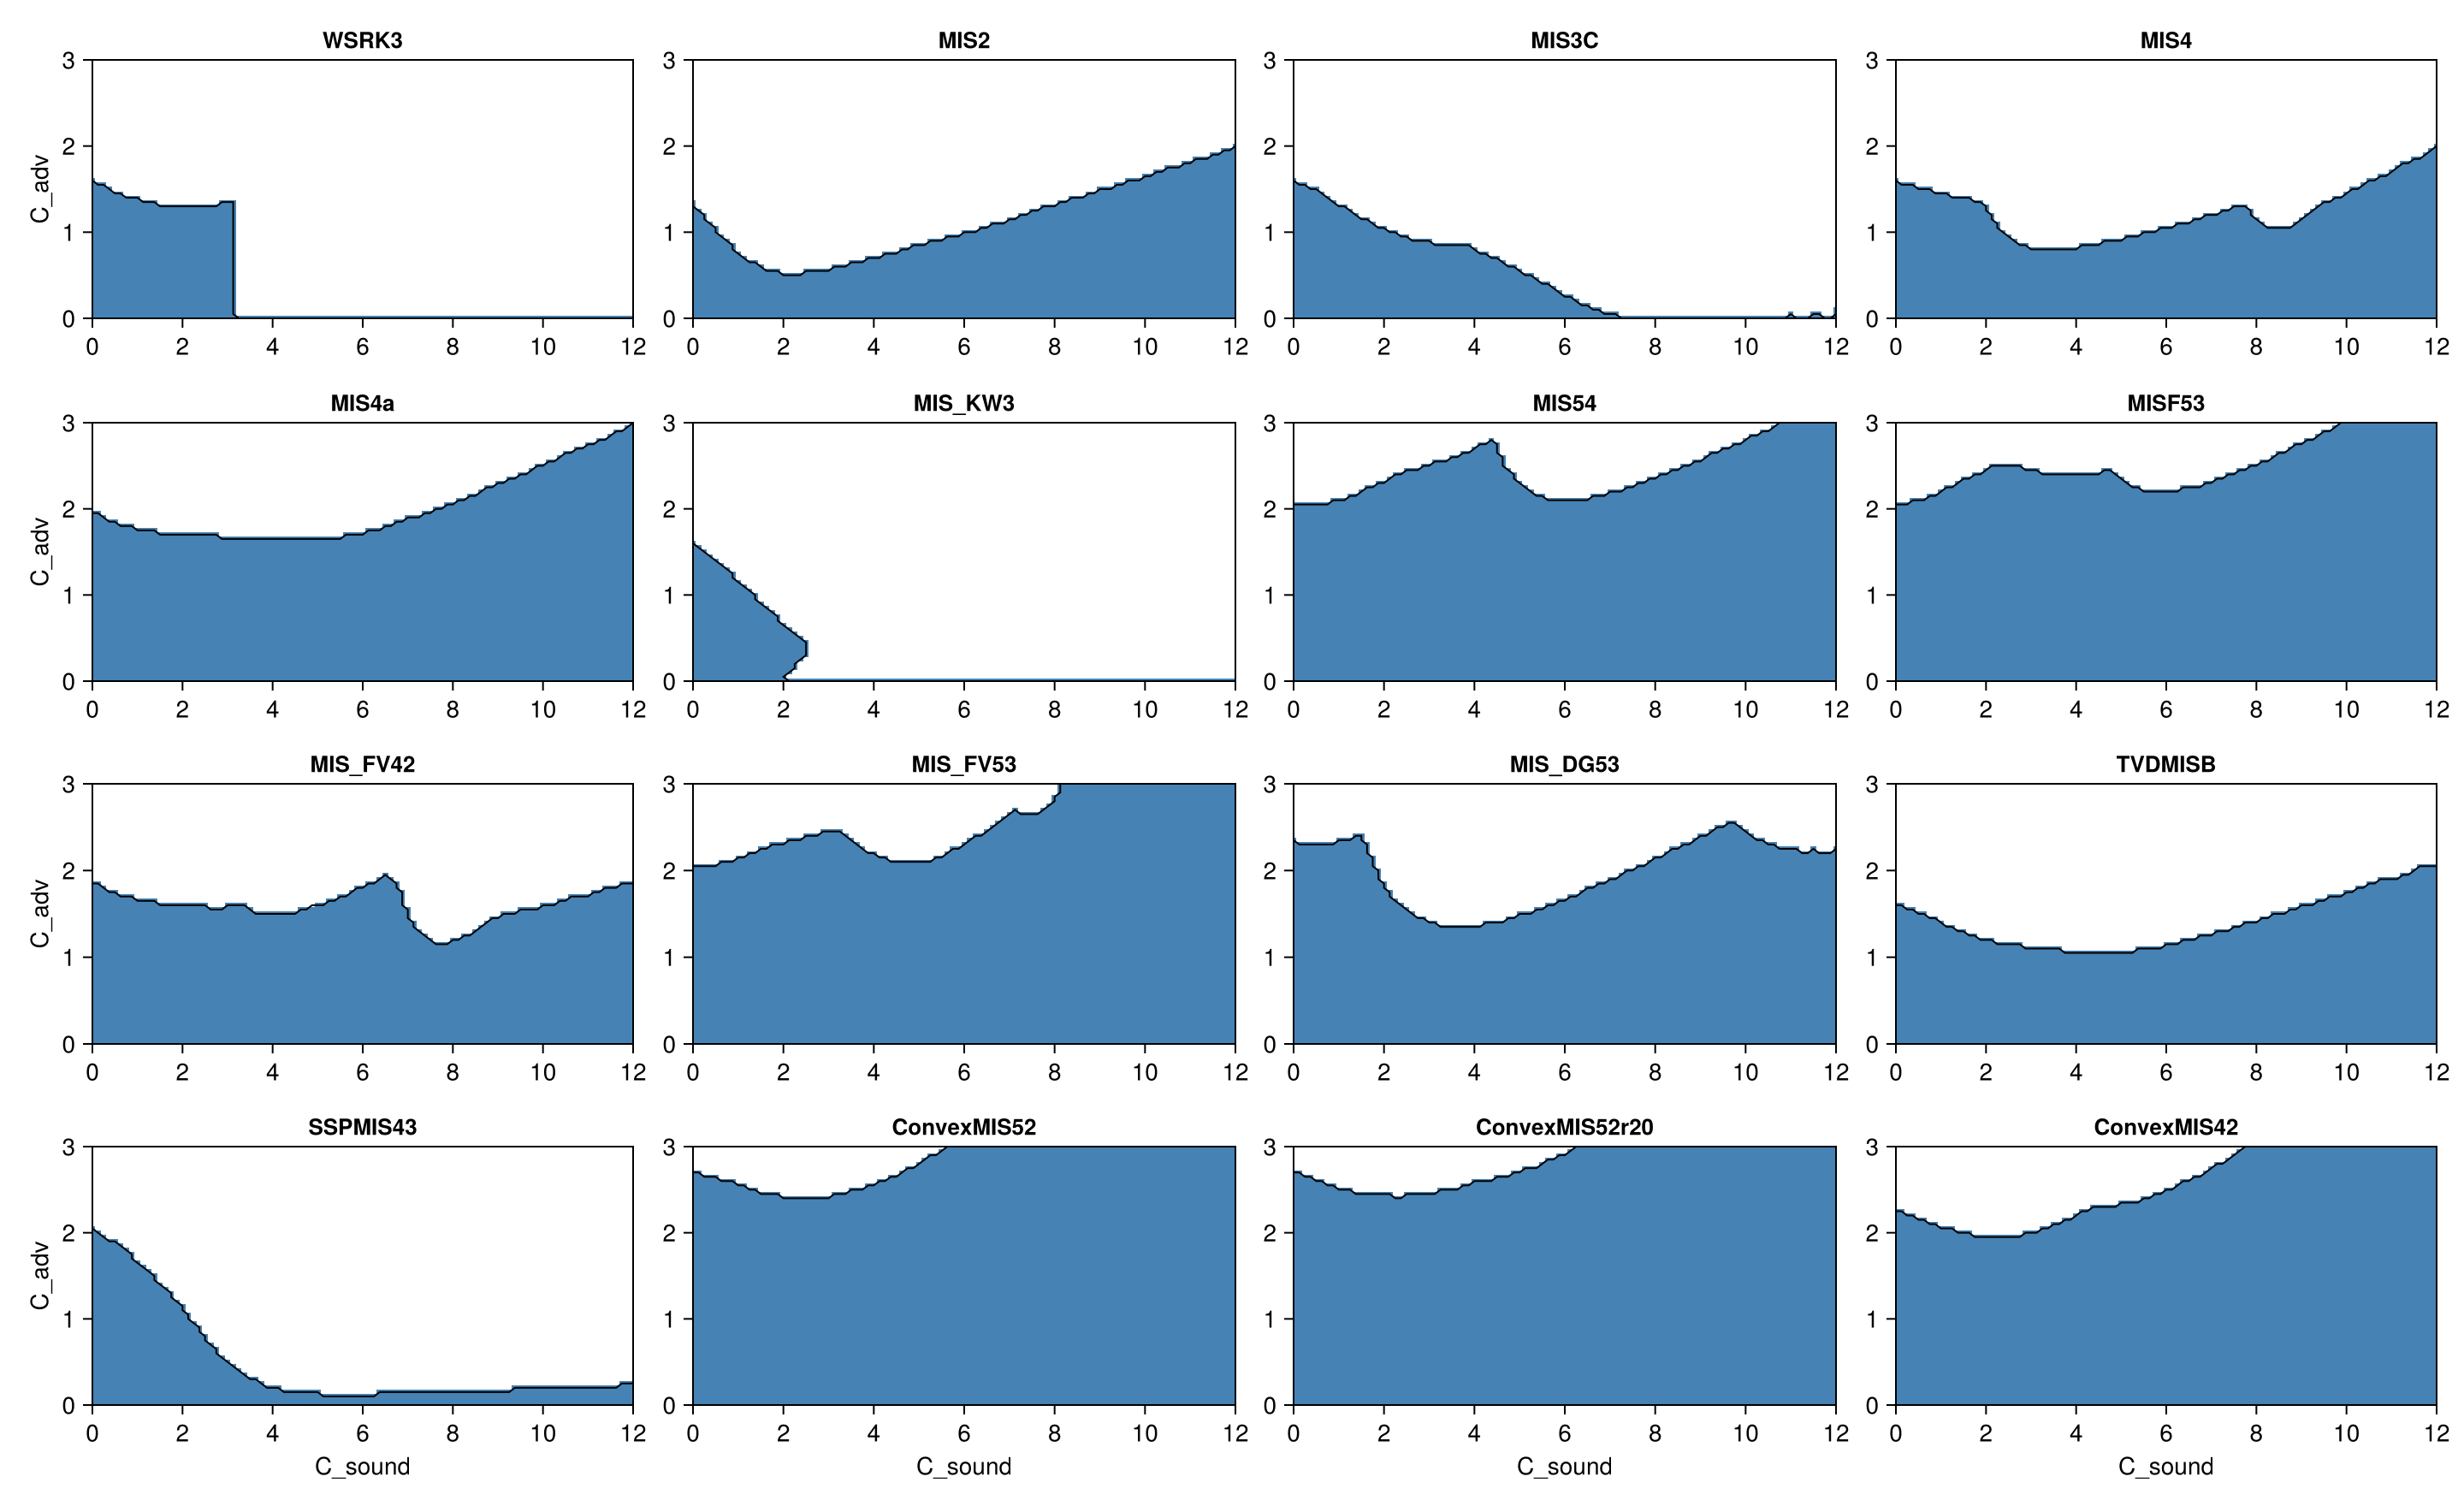
\includegraphics[width=\textwidth]{stability_fv/all.png}\end{center}
\tableofcontents
\clearpage
\section{WSRK3}
Wicker \& Skamarock (2002), RK3 split-explicit scheme: $\beta=\mathrm{diag}(1/3,1/2,1)$, $\alpha=\gamma=0$.

\noindent $s=3$, $\Sigma d=1.8333$, orders G/B/A/L: 2 / 2 / 2 / 2.\\ Stage times $c=(0.3333, 0.5000, 1.0000)$.

{\footnotesize\[(\alpha_{ij})_{i\ge2}=\left(\begin{array}{rr}0 & \\
0 & 0\end{array}\right)\]
\[\beta=\left(\begin{array}{rrr}0.3333333333 &  & \\
0 & 0.5000000000 & \\
0 & 0 & 1.0000000000\end{array}\right)\]
\[(\gamma_{ij})_{i\ge2}=\left(\begin{array}{rr}0 & \\
0 & 0\end{array}\right)\]}

\noindent Base Runge--Kutta method (\texttt{base\_method}; $F$ independent of its second argument), classical order 2:
{\footnotesize\[\begin{array}{r|rrr}0 &  &  & \\
0.3333333333 & 0.3333333333 &  & \\
0.5000000000 & 0 & 0.5000000000 & \\\hline
 & 0 & 0 & 1.0000000000\end{array}\]}

\begin{center}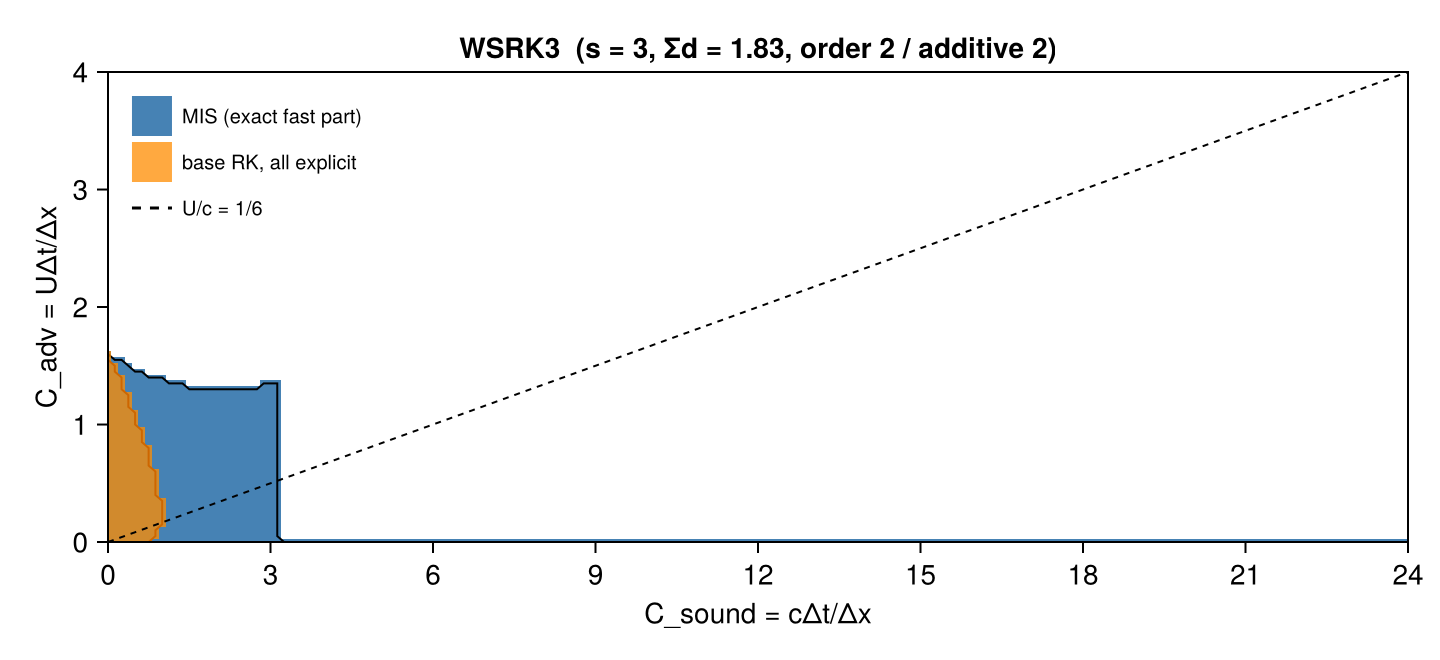
\includegraphics[width=0.8\textwidth]{stability_fv/WSRK3.png}

\small\begin{tabular}{lcccccccc}\toprule $C_{\rm sound}$ & 0 & 2 & 4 & 8 & 12 & 16 & 20 & 24\\\midrule largest $C_{\rm adv}$ & 1.60 & 1.30 & 0.00 & 0.00 & 0.00 & 0.00 & 0.00 & 0.00\\\bottomrule\end{tabular}\end{center}
\noindent On the line $U/c=1/6$ stable up to $C_{\rm sound}=3.12$ ($C_{\rm adv}=0.52$). Base Runge--Kutta method, all explicit: $C_{\rm adv}\le1.60$ at $C_{\rm sound}=0$, $C_{\rm sound}\le0.750$ at $C_{\rm adv}=0$.
\clearpage
\section{MIS2}
Knoth \& Wensch (2014).

\noindent $s=3$, $\Sigma d=1.1868$, orders G/B/A/L: 2 / 2 / 2 / 2.\\ Stage times $c=(0.1268, 0.7405, 1.0000)$.

{\footnotesize\[(\alpha_{ij})_{i\ge2}=\left(\begin{array}{rr}0.5369465667 & \\
0.4808929686 & 0.5005611636\end{array}\right)\]
\[\beta=\left(\begin{array}{rrr}0.1268484946 &  & \\
-0.7848382788 & 1.3744267527 & \\
-0.0456727082 & -0.0087508227 & 0.5247757886\end{array}\right)\]
\[(\gamma_{ij})_{i\ge2}=\left(\begin{array}{rr}0.6524651260 & \\
-0.0732769849 & 0.1449024304\end{array}\right)\]}

\noindent Base Runge--Kutta method (\texttt{base\_method}; $F$ independent of its second argument), classical order 2:
{\footnotesize\[\begin{array}{r|rrr}0 &  &  & \\
0.1268484946 & 0.1268484946 &  & \\
0.7404635565 & -0.6339631962 & 1.3744267527 & \\\hline
 & -0.4031673974 & 0.8783916087 & 0.5247757886\end{array}\]}

\begin{center}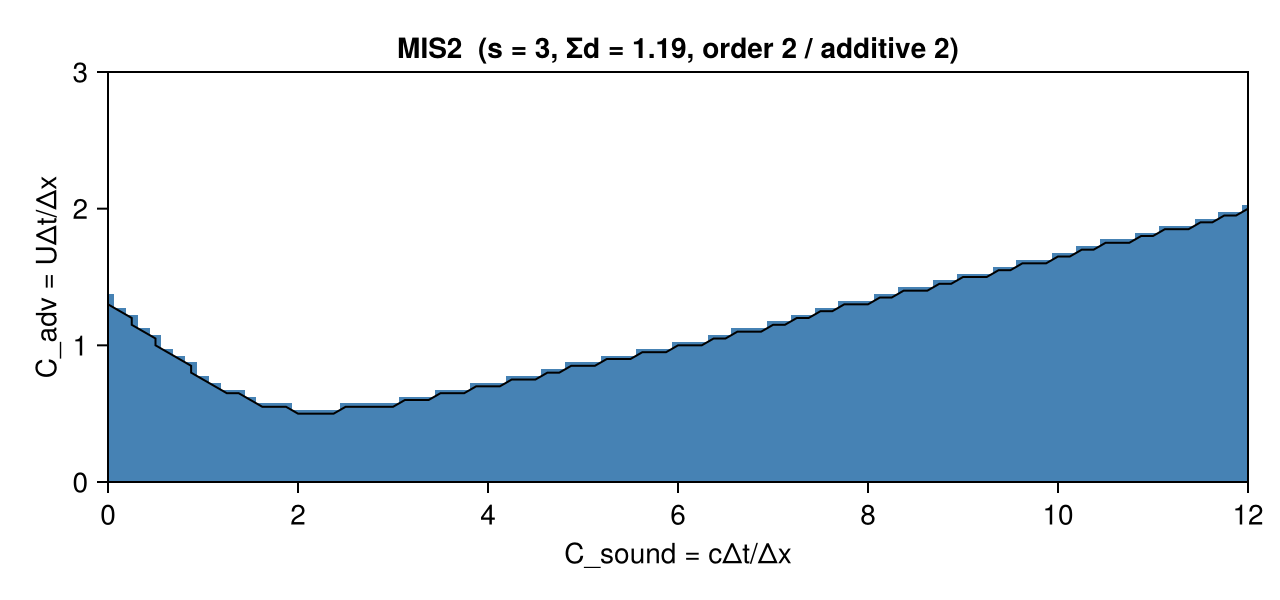
\includegraphics[width=0.8\textwidth]{stability_fv/MIS2.png}

\small\begin{tabular}{lcccccccc}\toprule $C_{\rm sound}$ & 0 & 2 & 4 & 8 & 12 & 16 & 20 & 24\\\midrule largest $C_{\rm adv}$ & 1.35 & 0.50 & 0.70 & 1.30 & 2.00 & 2.65 & 3.30 & 4.00\\\bottomrule\end{tabular}\end{center}
\noindent On the line $U/c=1/6$ stable up to $C_{\rm sound}=6.19$ ($C_{\rm adv}=1.03$). Base Runge--Kutta method, all explicit: $C_{\rm adv}\le1.35$ at $C_{\rm sound}=0$, $C_{\rm sound}\le0.000$ at $C_{\rm adv}=0$.
\clearpage
\section{MIS3C}
Knoth \& Wensch (2014).

\noindent $s=3$, $\Sigma d=1.1924$, orders G/B/A/L: 2 / 2 / 2 / 2.\\ Stage times $c=(0.3975, 0.6886, 1.0000)$.

{\footnotesize\[(\alpha_{ij})_{i\ge2}=\left(\begin{array}{rr}0.5895572771 & \\
0.5440366016 & 0.5655110426\end{array}\right)\]
\[\beta=\left(\begin{array}{rrr}0.3975251892 &  & \\
-0.2270364636 & 0.6245287946 & \\
-0.0029523808 & -0.2709717643 & 0.6713231594\end{array}\right)\]
\[(\gamma_{ij})_{i\ge2}=\left(\begin{array}{rr}0.1427987864 & \\
-0.0428918957 & 0.0202720980\end{array}\right)\]}

\noindent Base Runge--Kutta method (\texttt{base\_method}; $F$ independent of its second argument), classical order 3:
{\footnotesize\[\begin{array}{r|rrr}0 &  &  & \\
0.3975251892 & 0.3975251892 &  & \\
0.6886223137 & 0.0640935191 & 0.6245287946 & \\\hline
 & 0.2338101661 & 0.0948666744 & 0.6713231594\end{array}\]}

\begin{center}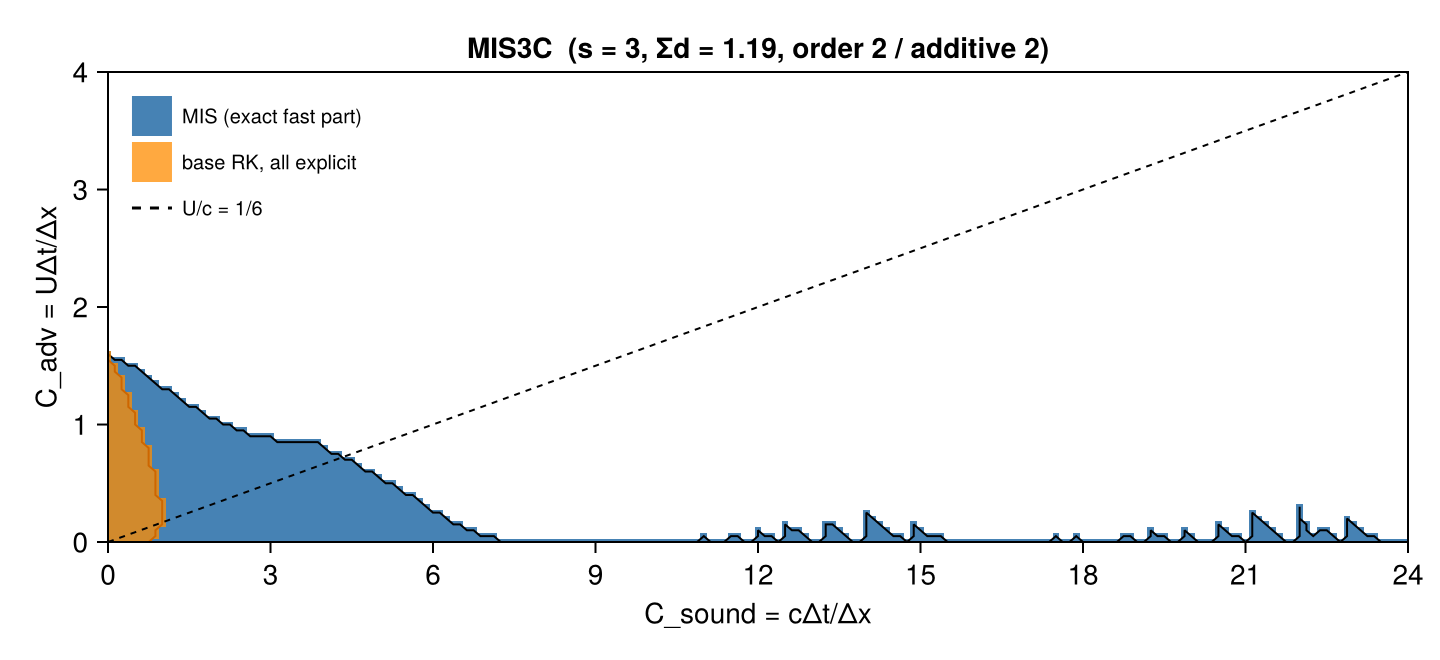
\includegraphics[width=0.8\textwidth]{stability_fv/MIS3C.png}

\small\begin{tabular}{lcccccccc}\toprule $C_{\rm sound}$ & 0 & 2 & 4 & 8 & 12 & 16 & 20 & 24\\\midrule largest $C_{\rm adv}$ & 1.60 & 1.05 & 0.80 & 0.00 & 0.10 & 0.00 & 0.05 & 0.00\\\bottomrule\end{tabular}\end{center}
\noindent On the line $U/c=1/6$ stable up to $C_{\rm sound}=4.38$ ($C_{\rm adv}=0.73$). Base Runge--Kutta method, all explicit: $C_{\rm adv}\le1.60$ at $C_{\rm sound}=0$, $C_{\rm sound}\le0.750$ at $C_{\rm adv}=0$.
\clearpage
\section{MIS4}
Knoth \& Wensch (2014).

\noindent $s=4$, $\Sigma d=1.4347$, orders G/B/A/L: 2 / 2 / 3 / 3.\\ Stage times $c=(0.1363, 0.4816, 0.5838, 1.0000)$.

{\footnotesize\[(\alpha_{ij})_{i\ge2}=\left(\begin{array}{rrr}0.9140928103 &  & \\
1.1427441740 & -0.2952112462 & \\
0.1129652822 & 0.3373694113 & 0.5037471831\end{array}\right)\]
\[\beta=\left(\begin{array}{rrrr}0.1362964784 &  &  & \\
0.2804623990 & -0.0160351334 &  & \\
0.9047133552 & -1.0401118315 & 0.6523375635 & \\
0.0671969846 & -0.3656218626 & -0.1548614708 & 0.9703624445\end{array}\right)\]
\[(\gamma_{ij})_{i\ge2}=\left(\begin{array}{rrr}0.6789519833 &  & \\
-1.3897416407 & 0.5038645763 & \\
-0.3753286083 & 0.3209250211 & -0.1582596889\end{array}\right)\]}

\noindent Base Runge--Kutta method (\texttt{base\_method}; $F$ independent of its second argument), classical order 3:
{\footnotesize\[\begin{array}{r|rrrr}0 &  &  &  & \\
0.1362964784 & 0.1362964784 &  &  & \\
0.4815536610 & 0.4975887943 & -0.0160351334 &  & \\
0.5837519772 & 0.9748720293 & -1.0434576155 & 0.6523375635 & \\\hline
 & 0.6958038146 & -0.7366792585 & 0.0705129993 & 0.9703624445\end{array}\]}

\begin{center}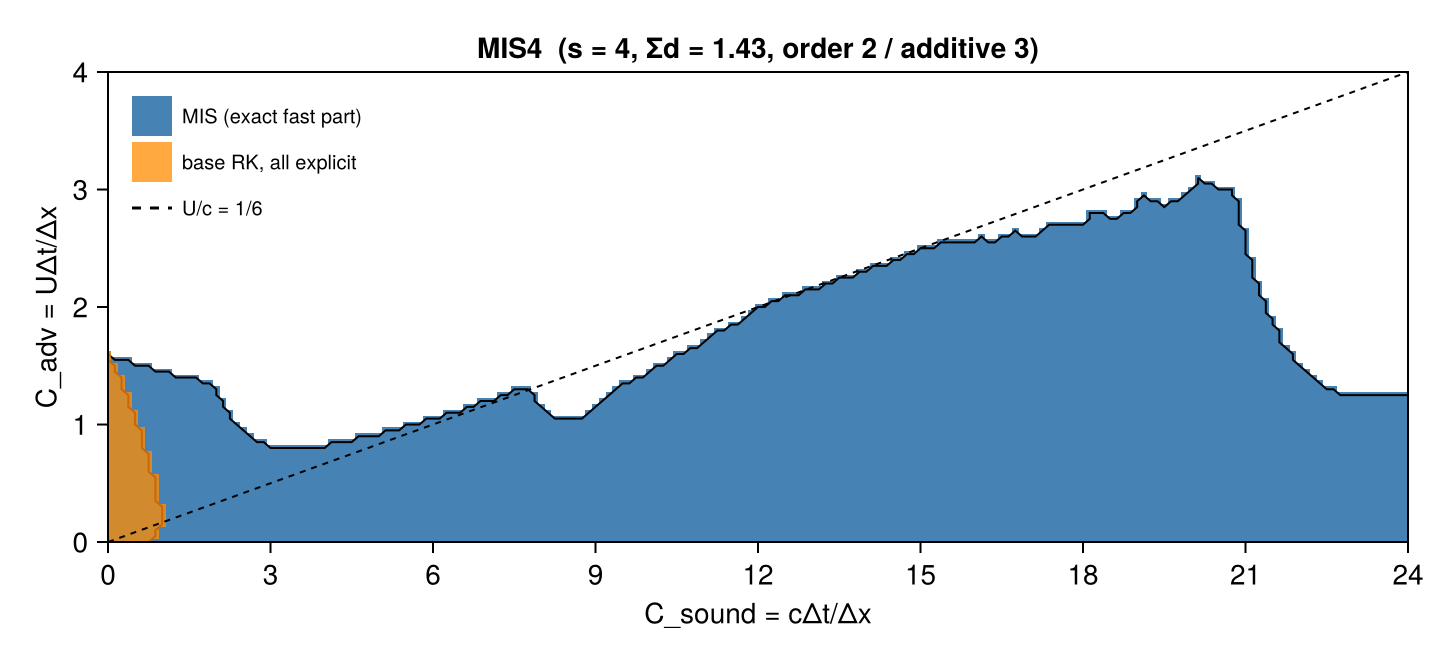
\includegraphics[width=0.8\textwidth]{stability_fv/MIS4.png}

\small\begin{tabular}{lcccccccc}\toprule $C_{\rm sound}$ & 0 & 2 & 4 & 8 & 12 & 16 & 20 & 24\\\midrule largest $C_{\rm adv}$ & 1.60 & 1.30 & 0.80 & 1.15 & 2.00 & 2.55 & 3.00 & 1.25\\\bottomrule\end{tabular}\end{center}
\noindent On the line $U/c=1/6$ stable up to $C_{\rm sound}=7.75$ ($C_{\rm adv}=1.29$). Base Runge--Kutta method, all explicit: $C_{\rm adv}\le1.60$ at $C_{\rm sound}=0$, $C_{\rm sound}\le0.750$ at $C_{\rm adv}=0$.
\clearpage
\section{MIS4a}
Knoth \& Wensch (2014), with the authors' corrected $\beta_{41}$ (values as in ClimaTimeSteppers.jl).

\noindent $s=4$, $\Sigma d=1.4719$, orders G/B/A/L: 2 / 2 / 3 / 3.\\ Stage times $c=(0.3876, 0.6152, 0.2325, 1.0000)$.

{\footnotesize\[(\alpha_{ij})_{i\ge2}=\left(\begin{array}{rrr}0.5234924992 &  & \\
1.1683374367 & -0.7576208024 & \\
-0.0364772338 & 0.5693614873 & 0.4774626300\end{array}\right)\]
\[\beta=\left(\begin{array}{rrrr}0.3875844464 &  &  & \\
-0.0253184484 & 0.3866894309 &  & \\
0.2089998352 & -0.4585664848 & 0.4342318757 & \\
-0.1004882220 & -0.4618617196 & 0.8304506212 & 0.2701491490\end{array}\right)\]
\[(\gamma_{ij})_{i\ge2}=\left(\begin{array}{rrr}0.1314508980 &  & \\
-0.3685585765 & 0.3315923264 & \\
-0.0657671305 & 0.0405910931 & 0.0649021116\end{array}\right)\]}

\noindent Base Runge--Kutta method (\texttt{base\_method}; $F$ independent of its second argument), classical order 3:
{\footnotesize\[\begin{array}{r|rrrr}0 &  &  &  & \\
0.3875844464 & 0.3875844464 &  &  & \\
0.6152168566 & 0.2285274257 & 0.3866894309 &  & \\
0.2325471732 & 0.4216224911 & -0.6233071937 & 0.4342318757 & \\\hline
 & 0.2279475191 & -0.5640593485 & 1.0659626803 & 0.2701491490\end{array}\]}

\begin{center}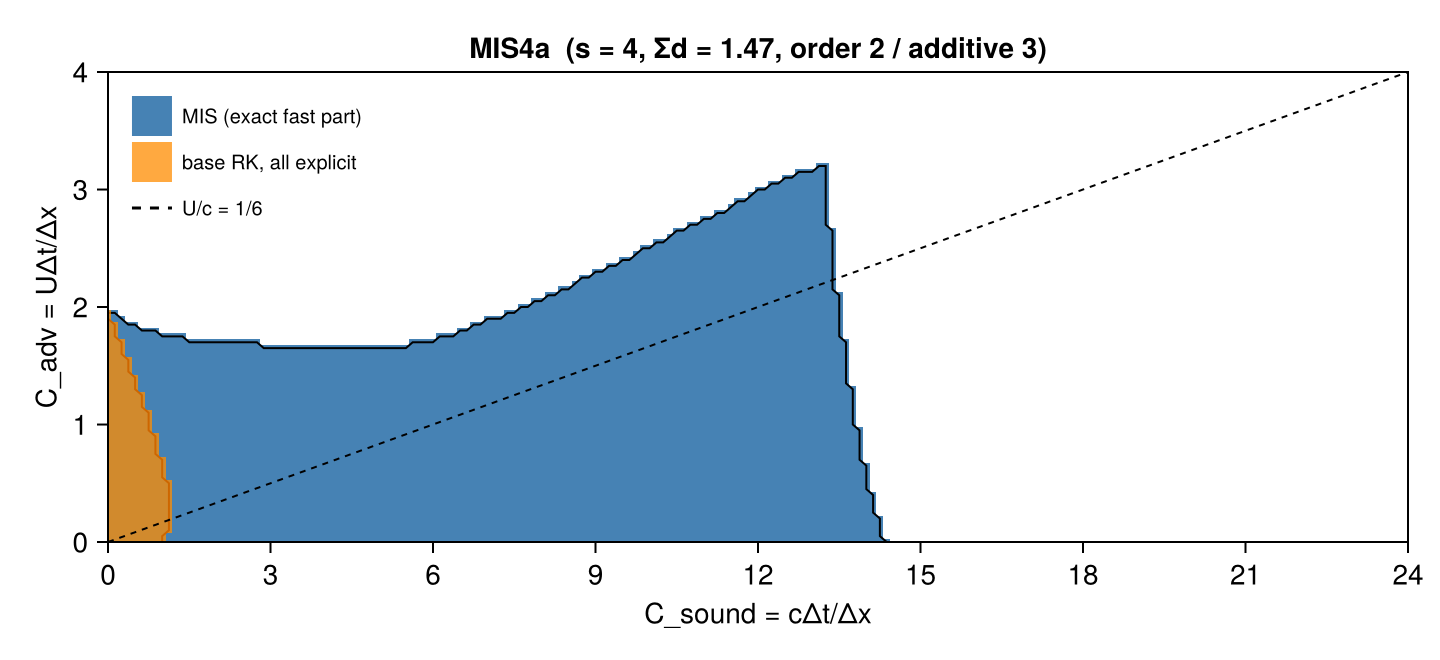
\includegraphics[width=0.8\textwidth]{stability_fv/MIS4a.png}

\small\begin{tabular}{lcccccccc}\toprule $C_{\rm sound}$ & 0 & 2 & 4 & 8 & 12 & 16 & 20 & 24\\\midrule largest $C_{\rm adv}$ & 1.95 & 1.70 & 1.65 & 2.05 & 3.00 & 0.00 & 0.00 & 0.00\\\bottomrule\end{tabular}\end{center}
\noindent On the line $U/c=1/6$ stable up to $C_{\rm sound}=13.44$ ($C_{\rm adv}=2.24$). Base Runge--Kutta method, all explicit: $C_{\rm adv}\le1.95$ at $C_{\rm sound}=0$, $C_{\rm sound}\le1.000$ at $C_{\rm adv}=0$.
\clearpage
\section{MIS\_KW3}
Knoth--Wolke RK3 ($c=0,1/3,3/4$) in MIS form with recursive stages ($\alpha_{i,i-1}=1$, $\gamma=0$).

\noindent $s=3$, $\Sigma d=1.0000$, orders G/B/A/L: 3 / 3 / 3 / 3.\\ Stage times $c=(0.3333, 0.7500, 1.0000)$.

{\footnotesize\[(\alpha_{ij})_{i\ge2}=\left(\begin{array}{rr}1.0000000000 & \\
0 & 1.0000000000\end{array}\right)\]
\[\beta=\left(\begin{array}{rrr}0.3333333333 &  & \\
-0.5208333333 & 0.9375000000 & \\
0.3541666667 & -0.6375000000 & 0.5333333333\end{array}\right)\]
\[(\gamma_{ij})_{i\ge2}=\left(\begin{array}{rr}0 & \\
0 & 0\end{array}\right)\]}

\noindent Base Runge--Kutta method (\texttt{base\_method}; $F$ independent of its second argument), classical order 3:
{\footnotesize\[\begin{array}{r|rrr}0 &  &  & \\
0.3333333333 & 0.3333333333 &  & \\
0.7500000000 & -0.1875000000 & 0.9375000000 & \\\hline
 & 0.1666666667 & 0.3000000000 & 0.5333333333\end{array}\]}

\begin{center}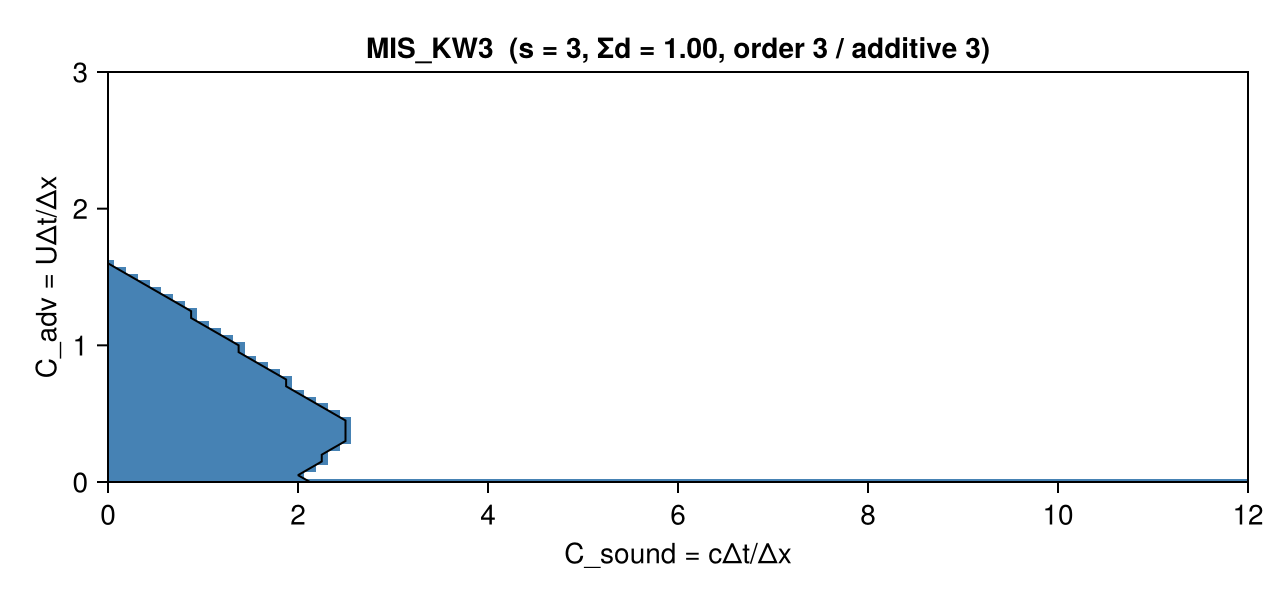
\includegraphics[width=0.8\textwidth]{stability_fv/MIS_KW3.png}

\small\begin{tabular}{lcccccccc}\toprule $C_{\rm sound}$ & 0 & 2 & 4 & 8 & 12 & 16 & 20 & 24\\\midrule largest $C_{\rm adv}$ & 1.60 & 0.65 & 0.00 & 0.00 & 0.00 & 0.00 & 0.00 & 0.00\\\bottomrule\end{tabular}\end{center}
\noindent On the line $U/c=1/6$ stable up to $C_{\rm sound}=2.50$ ($C_{\rm adv}=0.42$). Base Runge--Kutta method, all explicit: $C_{\rm adv}\le1.60$ at $C_{\rm sound}=0$, $C_{\rm sound}\le0.750$ at $C_{\rm adv}=0$.
\clearpage
\section{MIS54}
Bauer \& Knoth, J.~Comput.\ Appl.\ Math.\ 387 (2021), Table~2.

\noindent $s=5$, $\Sigma d=1.8778$, orders G/B/A/L: 2 / 2 / 4 / 4.\\ Stage times $c=(0.2196, 0.6184, 0.5301, 0.8081, 1.0000)$.

{\footnotesize\[(\alpha_{ij})_{i\ge2}=\left(\begin{array}{rrrr}0.0501434397 &  &  & \\
0.2875307202 & 0.2390308108 &  & \\
0.3826756599 & 0.1771856963 & -0.3148943836 & \\
0.0795916073 & 0.4598064016 & 0.0867252755 & 0.4399451963\end{array}\right)\]
\[\beta=\left(\begin{array}{rrrrr}0.2195793148 &  &  &  & \\
-0.0328649184 & 0.6346999188 &  &  & \\
-0.2417618874 & -0.1206315407 & 0.3746866208 &  & \\
-0.0584743241 & 0.3512172522 & 0.3096570302 & 0.1686047991 & \\
-0.0562050559 & -0.0683903310 & -0.0862092103 & 0.0349047056 & 0.4489649880\end{array}\right)\]
\[(\gamma_{ij})_{i\ge2}=\left(\begin{array}{rrrr}0.0255157040 &  &  & \\
0.2644454530 & 0.4022464824 &  & \\
-0.0682582968 & 0.0275586170 & 0.0158303686 & \\
0.0886109057 & 0.0678809828 & -0.2974161904 & 0.1482469092\end{array}\right)\]}

\noindent Base Runge--Kutta method (\texttt{base\_method}; $F$ independent of its second argument), classical order at least 4:
{\footnotesize\[\begin{array}{r|rrrrr}0 &  &  &  &  & \\
0.2195793148 & 0.2195793148 &  &  &  & \\
0.6184481833 & -0.0162517355 & 0.6346999188 &  &  & \\
0.5300925196 & -0.1309812065 & 0.2863871052 & 0.3746866208 &  & \\
0.8081364579 & 0.0464095401 & 0.3955203736 & 0.1976017450 & 0.1686047991 & \\\hline
 & 0.0270471762 & 0.4388356092 & -0.0489244908 & 0.1340767174 & 0.4489649880\end{array}\]}

\begin{center}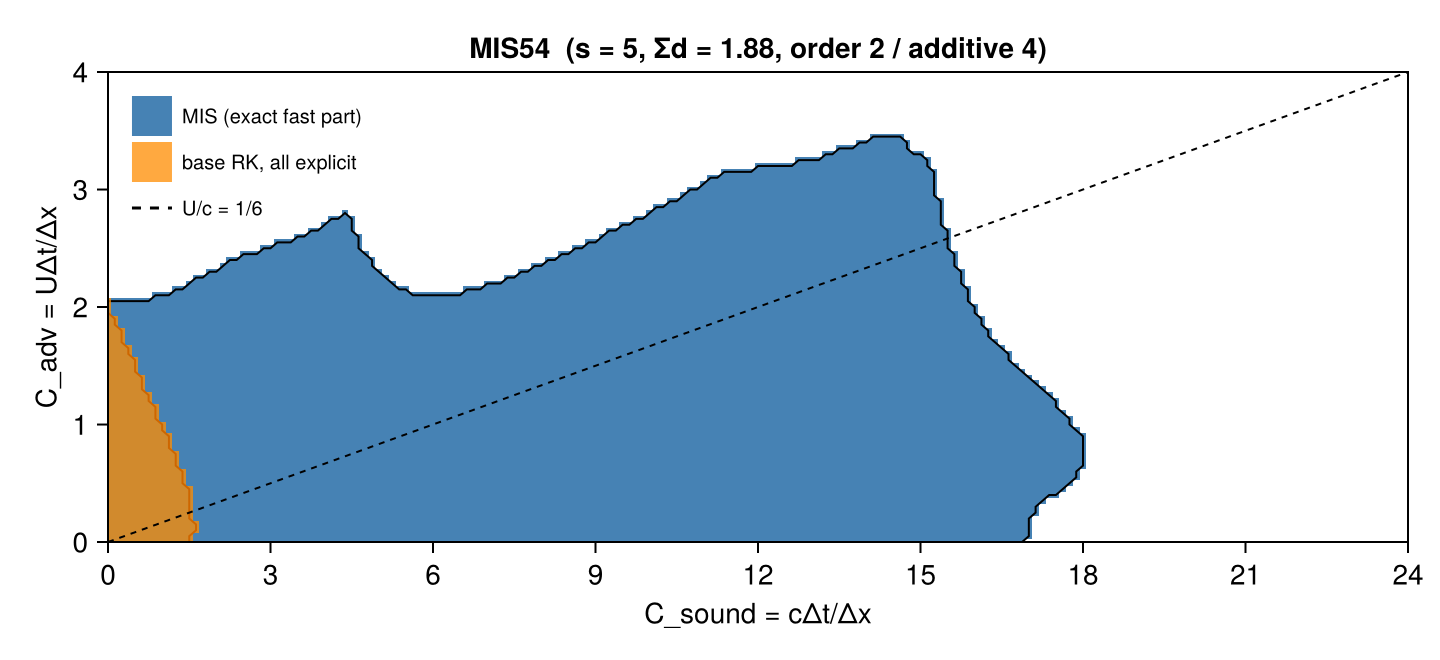
\includegraphics[width=0.8\textwidth]{stability_fv/MIS54.png}

\small\begin{tabular}{lcccccccc}\toprule $C_{\rm sound}$ & 0 & 2 & 4 & 8 & 12 & 16 & 20 & 24\\\midrule largest $C_{\rm adv}$ & 2.05 & 2.30 & 2.70 & 2.35 & 3.20 & 2.00 & 0.00 & 0.00\\\bottomrule\end{tabular}\end{center}
\noindent On the line $U/c=1/6$ stable up to $C_{\rm sound}=15.50$ ($C_{\rm adv}=2.58$). Base Runge--Kutta method, all explicit: $C_{\rm adv}\le2.05$ at $C_{\rm sound}=0$, $C_{\rm sound}\le1.500$ at $C_{\rm adv}=0$.
\clearpage
\section{MISF53}
This project (\texttt{MethodDesign/}): MIS54 projected (minimum norm) onto all bicoloured order conditions $\le3$.

\noindent $s=5$, $\Sigma d=1.9827$, orders G/B/A/L: 3 / 3 / 3 / 3.\\ Stage times $c=(0.2242, 0.6229, 0.6111, 0.8016, 1.0000)$.

{\footnotesize\[(\alpha_{ij})_{i\ge2}=\left(\begin{array}{rrrr}0.0515636909 &  &  & \\
0.2881762084 & 0.2373660404 &  & \\
0.3864261819 & 0.2268841207 & -0.3118830037 & \\
0.0713362061 & 0.4397591026 & 0.1006721717 & 0.4308139106\end{array}\right)\]
\[\beta=\left(\begin{array}{rrrrr}0.2241698201 &  &  &  & \\
-0.0309234741 & 0.6364492958 &  &  & \\
-0.2126611353 & -0.0906809281 & 0.4033420633 &  & \\
-0.0460277303 & 0.3549869064 & 0.3017520550 & 0.1641771597 & \\
-0.0398243639 & -0.0626545712 & -0.0929000637 & 0.0330415495 & 0.4404871895\end{array}\right)\]
\[(\gamma_{ij})_{i\ge2}=\left(\begin{array}{rrrr}0.0260551005 &  &  & \\
0.2597439218 & 0.3859110087 &  & \\
-0.0848120122 & 0.0175270451 & -0.0041962381 & \\
0.0851211659 & 0.0597321288 & -0.2562535272 & 0.1563916456\end{array}\right)\]}

\noindent Base Runge--Kutta method (\texttt{base\_method}; $F$ independent of its second argument), classical order 3:
{\footnotesize\[\begin{array}{r|rrrrr}0 &  &  &  &  & \\
0.2241698201 & 0.2241698201 &  &  &  & \\
0.6229256122 & -0.0135236836 & 0.6364492958 &  &  & \\
0.6110823944 & -0.0982629799 & 0.3060033109 & 0.4033420633 &  & \\
0.8016007001 & 0.0493386128 & 0.4138209262 & 0.1742640014 & 0.1641771597 & \\\hline
 & 0.0327534908 & 0.4506358085 & -0.0533237787 & 0.1294472899 & 0.4404871895\end{array}\]}

\begin{center}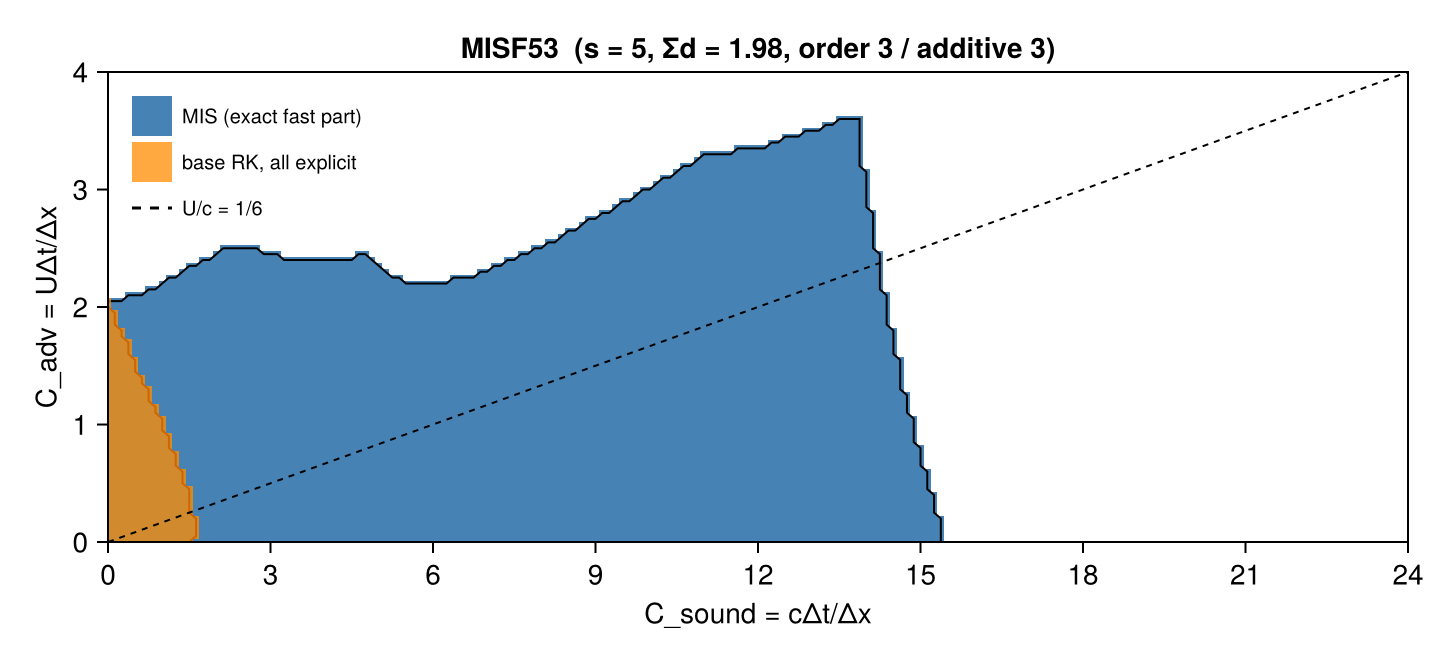
\includegraphics[width=0.8\textwidth]{stability_fv/MISF53.png}

\small\begin{tabular}{lcccccccc}\toprule $C_{\rm sound}$ & 0 & 2 & 4 & 8 & 12 & 16 & 20 & 24\\\midrule largest $C_{\rm adv}$ & 2.05 & 2.45 & 2.40 & 2.50 & 3.35 & 0.00 & 0.00 & 0.00\\\bottomrule\end{tabular}\end{center}
\noindent On the line $U/c=1/6$ stable up to $C_{\rm sound}=14.25$ ($C_{\rm adv}=2.38$). Base Runge--Kutta method, all explicit: $C_{\rm adv}\le2.05$ at $C_{\rm sound}=0$, $C_{\rm sound}\le1.500$ at $C_{\rm adv}=0$.
\clearpage
\section{MIS\_FV42}
This project (\texttt{MethodDesign/search\_app.jl}): from MIS4, stable on the column Fourier blocks of the frozen FV split.

\noindent $s=4$, $\Sigma d=1.3760$, orders G/B/A/L: 2 / 2 / 2 / 2.\\ Stage times $c=(0.1003, 0.3395, 0.4630, 1.0000)$.

{\footnotesize\[(\alpha_{ij})_{i\ge2}=\left(\begin{array}{rrr}0.9395339038 &  & \\
0.7145447566 & -0.0700821608 & \\
0.2087031282 & 0.3326186904 & 0.4629378742\end{array}\right)\]
\[\beta=\left(\begin{array}{rrrr}0.1003256765 &  &  & \\
0.0763381182 & 0.0908553402 &  & \\
0.8827006045 & -1.0884801915 & 0.6700284267 & \\
-0.0676742586 & -0.3359696330 & -0.0892733264 & 1.1371806399\end{array}\right)\]
\[(\gamma_{ij})_{i\ge2}=\left(\begin{array}{rrr}0.7777109910 &  & \\
-2.0872818089 & 0.4722290177 & \\
-0.3908340955 & 0.4277396917 & -0.2126728799\end{array}\right)\]}

\noindent Base Runge--Kutta method (\texttt{base\_method}; $F$ independent of its second argument), classical order 2:
{\footnotesize\[\begin{array}{r|rrrr}0 &  &  &  & \\
0.1003256765 & 0.1003256765 &  &  & \\
0.3394772143 & 0.2486218740 & 0.0908553402 &  & \\
0.4630477609 & 0.8449623362 & -1.0519430020 & 0.6700284267 & \\\hline
 & 0.3145595491 & -0.5301515229 & 0.0784113340 & 1.1371806399\end{array}\]}

\begin{center}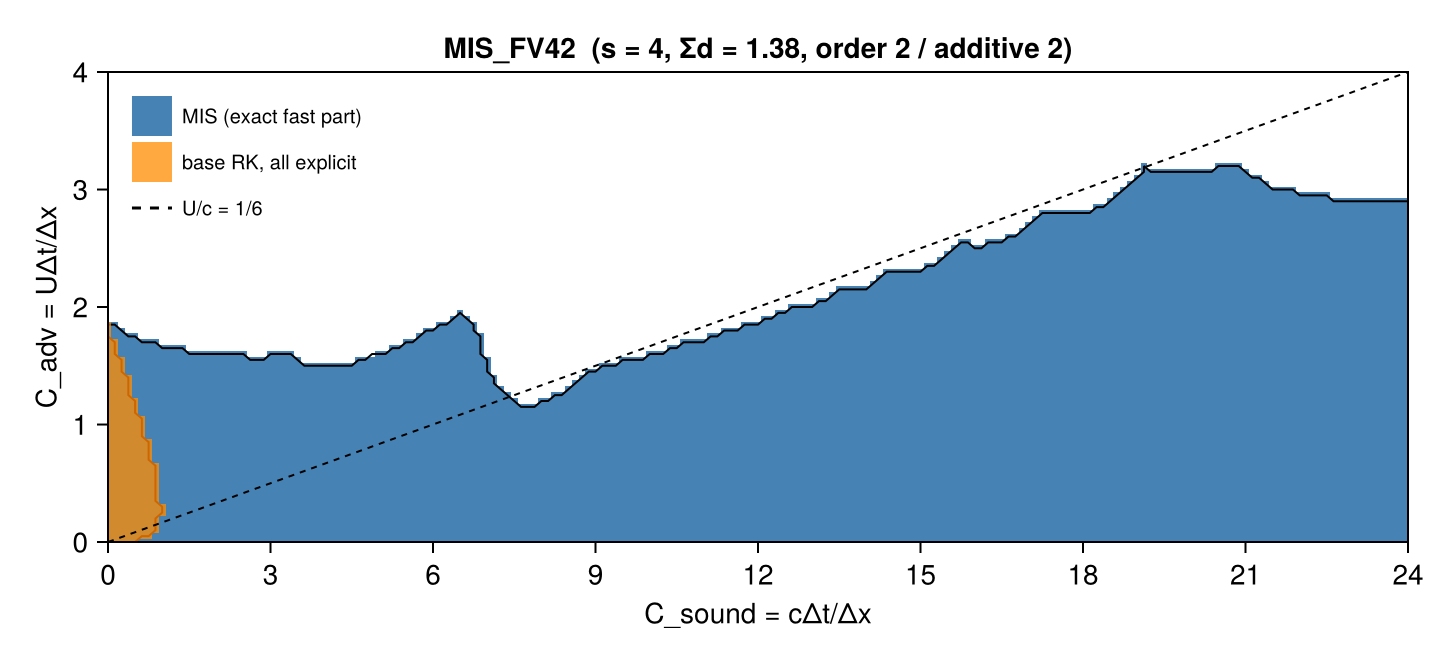
\includegraphics[width=0.8\textwidth]{stability_fv/MIS_FV42.png}

\small\begin{tabular}{lcccccccc}\toprule $C_{\rm sound}$ & 0 & 2 & 4 & 8 & 12 & 16 & 20 & 24\\\midrule largest $C_{\rm adv}$ & 1.85 & 1.60 & 1.50 & 1.20 & 1.85 & 2.50 & 3.15 & 2.90\\\bottomrule\end{tabular}\end{center}
\noindent On the line $U/c=1/6$ stable up to $C_{\rm sound}=7.38$ ($C_{\rm adv}=1.23$). Base Runge--Kutta method, all explicit: $C_{\rm adv}\le1.85$ at $C_{\rm sound}=0$, $C_{\rm sound}\le0.500$ at $C_{\rm adv}=0$.
\clearpage
\section{MIS\_FV53}
This project (\texttt{MethodDesign/search\_app.jl}): from MISF53, stable on the column Fourier blocks of the frozen FV split.

\noindent $s=5$, $\Sigma d=2.0672$, orders G/B/A/L: 3 / 3 / 3 / 3.\\ Stage times $c=(0.2041, 0.6026, 0.6842, 0.7615, 1.0000)$.

{\footnotesize\[(\alpha_{ij})_{i\ge2}=\left(\begin{array}{rrrr}0.0440307746 &  &  & \\
0.2668396897 & 0.2440553703 &  & \\
0.4352306171 & 0.2524288435 & -0.2614776416 & \\
0.0808872063 & 0.4761807415 & 0.1003632036 & 0.3573909626\end{array}\right)\]
\[\beta=\left(\begin{array}{rrrrr}0.2041341365 &  &  &  & \\
-0.0549344783 & 0.6435699077 &  &  & \\
-0.1692526404 & -0.0768629275 & 0.4557029326 &  & \\
-0.0550264662 & 0.3608672029 & 0.2788260922 & 0.1448719005 & \\
-0.0256011149 & -0.0747751758 & -0.1224620391 & 0.0254765996 & 0.5326201034\end{array}\right)\]
\[(\gamma_{ij})_{i\ge2}=\left(\begin{array}{rrrr}0.0242157334 &  &  & \\
0.2508100147 & 0.3681510161 &  & \\
-0.0901380731 & 0.0092768617 & -0.0252006568 & \\
0.0955669275 & 0.0914326157 & -0.2473031202 & 0.1510811987\end{array}\right)\]}

\noindent Base Runge--Kutta method (\texttt{base\_method}; $F$ independent of its second argument), classical order 3:
{\footnotesize\[\begin{array}{r|rrrrr}0 &  &  &  &  & \\
0.2041341365 & 0.2041341365 &  &  &  & \\
0.6025668713 & -0.0410030363 & 0.6435699077 &  &  & \\
0.6841526270 & -0.0886849857 & 0.3171346800 & 0.4557029326 &  & \\
0.7615473749 & 0.0301120346 & 0.4383774890 & 0.1481859509 & 0.1448719005 & \\\hline
 & 0.0154878219 & 0.4668267060 & -0.1140745592 & 0.0991399280 & 0.5326201034\end{array}\]}

\begin{center}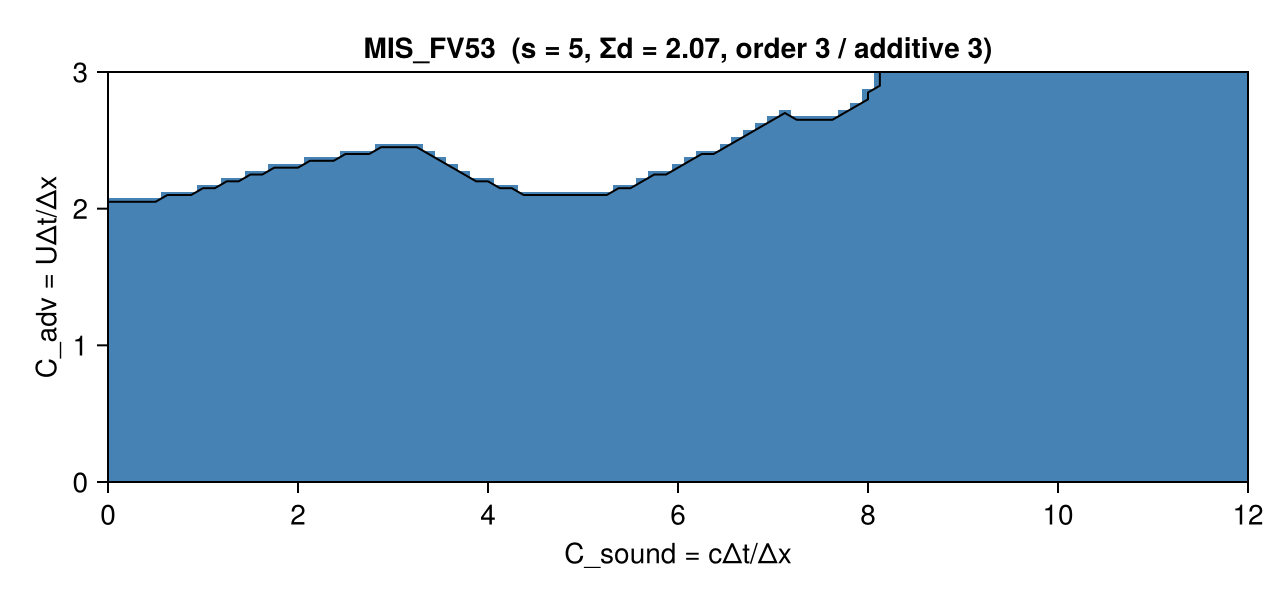
\includegraphics[width=0.8\textwidth]{stability_fv/MIS_FV53.png}

\small\begin{tabular}{lcccccccc}\toprule $C_{\rm sound}$ & 0 & 2 & 4 & 8 & 12 & 16 & 20 & 24\\\midrule largest $C_{\rm adv}$ & 2.05 & 2.30 & 2.20 & 2.85 & 4.00 & 2.95 & 3.30 & 4.00\\\bottomrule\end{tabular}\end{center}
\noindent On the line $U/c=1/6$ stable up to $C_{\rm sound}=17.56$ ($C_{\rm adv}=2.93$). Base Runge--Kutta method, all explicit: $C_{\rm adv}\le2.05$ at $C_{\rm sound}=0$, $C_{\rm sound}\le0.000$ at $C_{\rm adv}=0$.
\clearpage
\section{MIS\_DG53}
This project (\texttt{MethodDesign/search\_app.jl}): from MISF53, stable on the column Fourier blocks of the frozen DG split.

\noindent $s=5$, $\Sigma d=1.9176$, orders G/B/A/L: 3 / 3 / 3 / 3.\\ Stage times $c=(0.2431, 0.5738, 0.6043, 0.8459, 1.0000)$.

{\footnotesize\[(\alpha_{ij})_{i\ge2}=\left(\begin{array}{rrrr}0.0503566658 &  &  & \\
0.2060869552 & 0.2904943302 &  & \\
0.8037586634 & 0.1618443192 & -0.2604741095 & \\
0.1310475468 & 0.4728849533 & 0.2251726454 & 0.2666117026\end{array}\right)\]
\[\beta=\left(\begin{array}{rrrrr}0.2430523989 &  &  &  & \\
0.0175409351 & 0.5308221928 &  &  & \\
-0.1539877508 & -0.0785018232 & 0.3324895740 &  & \\
-0.1859532840 & 0.4937758316 & 0.2382121745 & 0.2043648283 & \\
-0.0081736253 & -0.0599699445 & -0.1074159266 & 0.1230330052 & 0.3283073405\end{array}\right)\]
\[(\gamma_{ij})_{i\ge2}=\left(\begin{array}{rrrr}0.0544043021 &  &  & \\
0.1429257541 & 0.4404706150 &  & \\
-0.0998023777 & -0.0248617089 & 0.0052525944 & \\
0.0507762742 & -0.0595883487 & -0.2887211160 & 0.3023438824\end{array}\right)\]}

\noindent Base Runge--Kutta method (\texttt{base\_method}; $F$ independent of its second argument), classical order 3:
{\footnotesize\[\begin{array}{r|rrrrr}0 &  &  &  &  & \\
0.2430523989 & 0.2430523989 &  &  &  & \\
0.5738255324 & 0.0430033396 & 0.5308221928 &  &  & \\
0.6042747251 & -0.0377254407 & 0.3095105919 & 0.3324895740 &  & \\
0.8458780228 & 0.0006640339 & 0.4874954790 & 0.1533536816 & 0.2043648283 & \\\hline
 & 0.0565674247 & 0.4171114160 & -0.0412936969 & 0.2393075156 & 0.3283073405\end{array}\]}

\begin{center}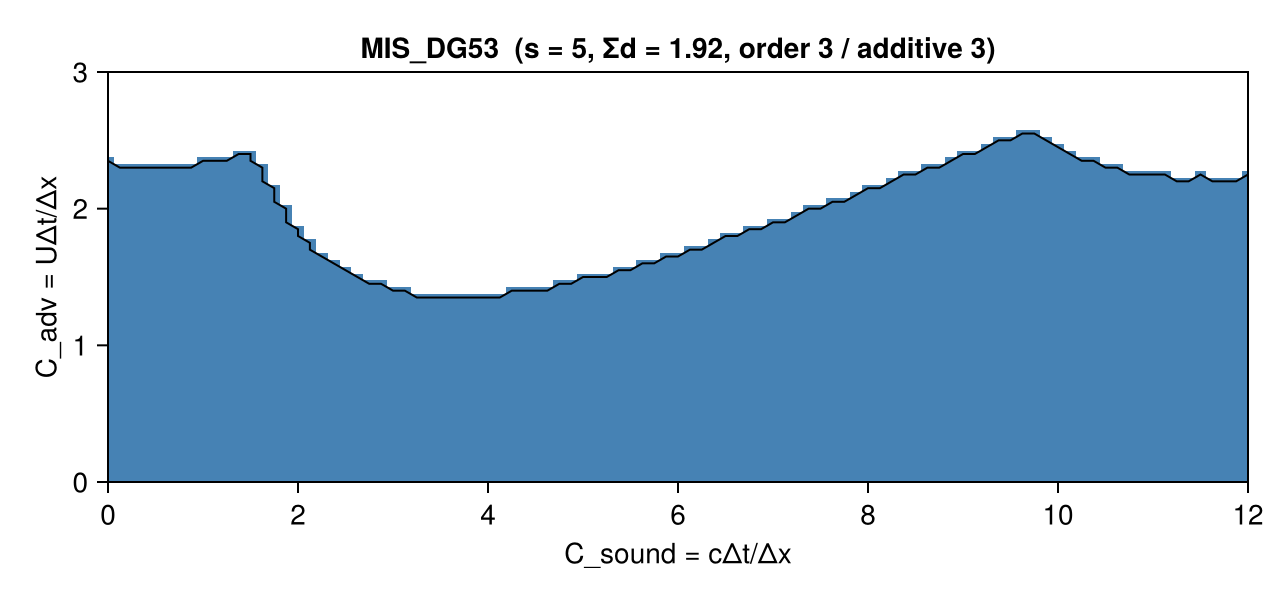
\includegraphics[width=0.8\textwidth]{stability_fv/MIS_DG53.png}

\small\begin{tabular}{lcccccccc}\toprule $C_{\rm sound}$ & 0 & 2 & 4 & 8 & 12 & 16 & 20 & 24\\\midrule largest $C_{\rm adv}$ & 2.35 & 1.85 & 1.35 & 2.15 & 2.25 & 2.70 & 2.85 & 2.40\\\bottomrule\end{tabular}\end{center}
\noindent On the line $U/c=1/6$ stable up to $C_{\rm sound}=15.31$ ($C_{\rm adv}=2.55$). Base Runge--Kutta method, all explicit: $C_{\rm adv}\le2.35$ at $C_{\rm sound}=0$, $C_{\rm sound}\le1.375$ at $C_{\rm adv}=0$.
\clearpage
\section{TVDMISB}
Knoth \& Wensch (2014), as in Breeze.jl. The published coefficients have about 6 digits: the residual of \(\bullet[w]\) is \(2\cdot10^{-6}\).

\noindent $s=3$, $\Sigma d=1.2684$, orders G/B/A/L: 2 / 2 / 2 / 2.\\ Stage times $c=(0.6667, 0.6667, 1.0000)$.

{\footnotesize\[(\alpha_{ij})_{i\ge2}=\left(\begin{array}{rr}0.4266823286 & \\
0.2657077902 & 0.4148996689\end{array}\right)\]
\[\beta=\left(\begin{array}{rrr}0.6666666667 &  & \\
-0.2549285910 & 0.4444444444 & \\
-0.2645251718 & 0.1142408442 & 0.5625000000\end{array}\right)\]
\[(\gamma_{ij})_{i\ge2}=\left(\begin{array}{rr}0.2890438912 & \\
0.4511356007 & -0.2500665685\end{array}\right)\]}

\noindent Base Runge--Kutta method (\texttt{base\_method}; $F$ independent of its second argument), classical order 3:
{\footnotesize\[\begin{array}{r|rrr}0 &  &  & \\
0.6666666667 & 0.6666666667 &  & \\
0.6666666667 & 0.2222222222 & 0.4444444444 & \\\hline
 & 0.2500000000 & 0.1875000000 & 0.5625000000\end{array}\]}

\begin{center}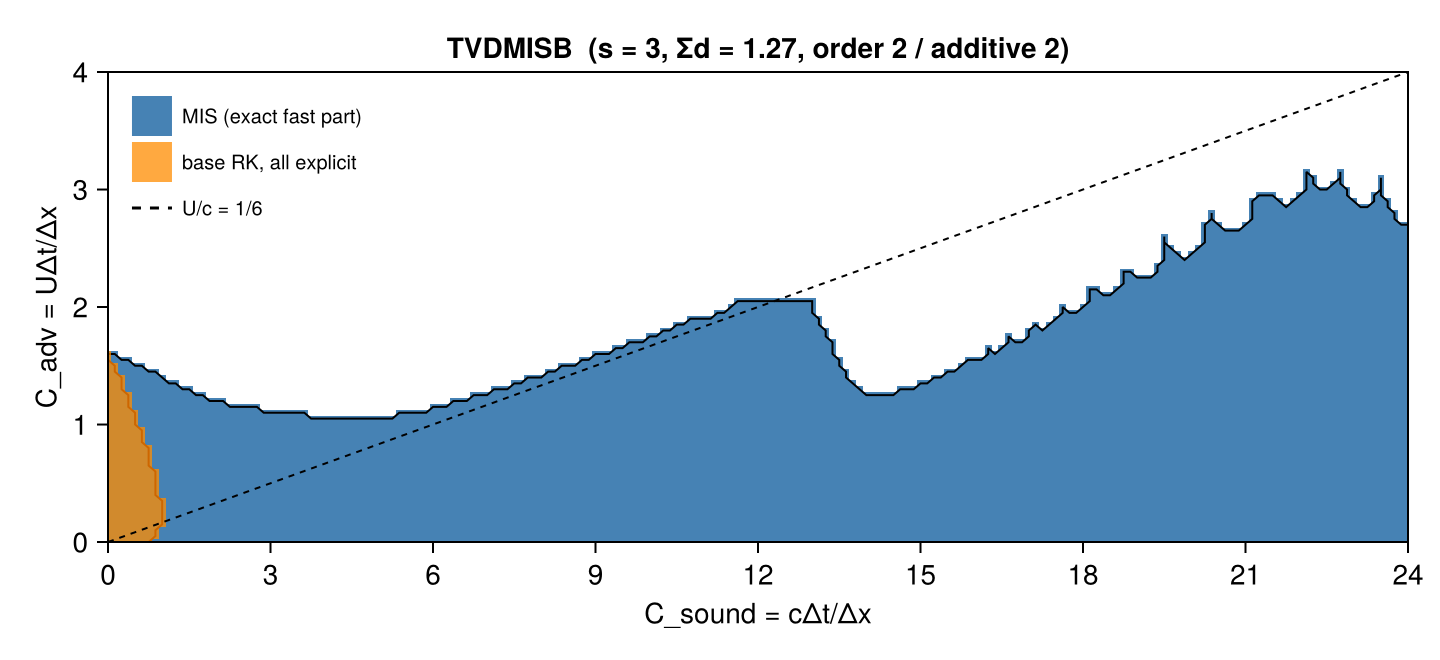
\includegraphics[width=0.8\textwidth]{stability_fv/TVDMISB.png}

\small\begin{tabular}{lcccccccc}\toprule $C_{\rm sound}$ & 0 & 2 & 4 & 8 & 12 & 16 & 20 & 24\\\midrule largest $C_{\rm adv}$ & 1.60 & 1.20 & 1.05 & 1.40 & 2.05 & 1.55 & 2.45 & 2.70\\\bottomrule\end{tabular}\end{center}
\noindent On the line $U/c=1/6$ stable up to $C_{\rm sound}=12.31$ ($C_{\rm adv}=2.05$). Base Runge--Kutta method, all explicit: $C_{\rm adv}\le1.60$ at $C_{\rm sound}=0$, $C_{\rm sound}\le0.750$ at $C_{\rm adv}=0$.
\clearpage
\section{SSPMIS43}
Breeze.jl (branch \texttt{glw/mis-tableau-search}): coupled order 2, slow order 3, SSP slow method (SSP coefficient 1.79), CMA-ES search for the cost per simulated time with Breeze's own fast integrator.

\noindent $s=4$, $\Sigma d=1.1405$, orders G/B/A/L: 2 / 2 / 2 / 2.\\ Stage times $c=(0.5598, 0.8981, 0.5713, 1.0000)$.

{\footnotesize\[(\alpha_{ij})_{i\ge2}=\left(\begin{array}{rrr}0.6272449216 &  & \\
0.2343016429 & 1.0654114266 & \\
0.0044647991 & 0.4767621383 & 0.3406131794\end{array}\right)\]
\[\beta=\left(\begin{array}{rrrr}0.5597870483 &  &  & \\
-0.1370337470 & 0.4455138059 &  & \\
-0.0835605665 & 0.0113565878 & 0.2115744905 & \\
-0.0771783999 & -0.2829502200 & 0.0540345576 & 0.4389305930\end{array}\right)\]
\[(\gamma_{ij})_{i\ge2}=\left(\begin{array}{rrr}0.4259875231 &  & \\
-0.0338865442 & -0.7094153778 & \\
-0.3331958955 & 0.3558111250 & 0.1906209780\end{array}\right)\]}

\noindent Base Runge--Kutta method (\texttt{base\_method}; $F$ independent of its second argument), classical order 3:
{\footnotesize\[\begin{array}{r|rrrr}0 &  &  &  & \\
0.5597870483 & 0.5597870483 &  &  & \\
0.8980659404 & 0.4525521345 & 0.4455138059 &  & \\
0.5712682147 & 0.1897359818 & 0.1699577424 & 0.2115744905 & \\\hline
 & 0.2163792318 & 0.1782600213 & 0.1664301538 & 0.4389305930\end{array}\]}

\begin{center}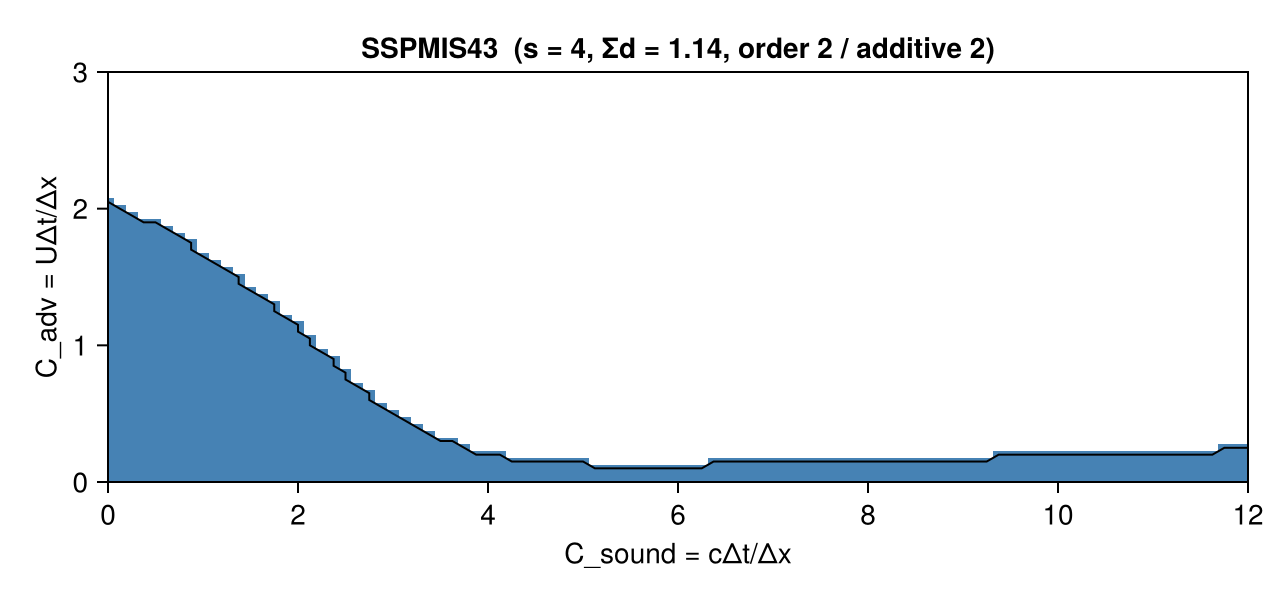
\includegraphics[width=0.8\textwidth]{stability_fv/SSPMIS43.png}

\small\begin{tabular}{lcccccccc}\toprule $C_{\rm sound}$ & 0 & 2 & 4 & 8 & 12 & 16 & 20 & 24\\\midrule largest $C_{\rm adv}$ & 2.05 & 1.15 & 0.20 & 0.15 & 0.25 & 0.35 & 0.45 & 0.55\\\bottomrule\end{tabular}\end{center}
\noindent On the line $U/c=1/6$ stable up to $C_{\rm sound}=3.00$ ($C_{\rm adv}=0.50$). Base Runge--Kutta method, all explicit: $C_{\rm adv}\le2.05$ at $C_{\rm sound}=0$, $C_{\rm sound}\le1.000$ at $C_{\rm adv}=0$.
\clearpage
\section{ConvexMIS52}
Breeze.jl (branch \texttt{glw/mis-tableau-search}): coupled order 2, convex stage start states, $\beta\ge0$, Shu--Osher coefficient 1.5; constrained search for the stable step per cost.

\noindent $s=5$, $\Sigma d=1.8252$, orders G/B/A/L: 2 / 2 / 2 / 2.\\ Stage times $c=(0.6061, 0.4508, 0.6387, 1.0393, 1.0000)$.

{\footnotesize\[(\alpha_{ij})_{i\ge2}=\left(\begin{array}{rrrr}0.0271061564 &  &  & \\
0.0671888783 & 0.4736160731 &  & \\
0.1031101522 & 0.6430040031 & 0.0898518700 & \\
0.1166337029 & 0.2375505711 & 0.3911029005 & 0.0793221893\end{array}\right)\]
\[\beta=\left(\begin{array}{rrrrr}0.6060736559 &  &  &  & \\
0.0011868577 & 0.2344852294 &  &  & \\
0.0026173419 & 0.0010473060 & 0.2932696268 &  & \\
0.0077634772 & 0.0311973908 & 0.0016270376 & 0.4117588484 & \\
0.0005343085 & 0.0037687547 & 0.0020199481 & 0.0010348065 & 0.2267946458\end{array}\right)\]
\[(\gamma_{ij})_{i\ge2}=\left(\begin{array}{rrrr}0.3278316115 &  &  & \\
0.1638434139 & -0.0261473918 &  & \\
0.0917166006 & -0.4855126788 & 0.5330677474 & \\
-0.0513968489 & -0.2054019354 & 0.1652916797 & 0.2636743706\end{array}\right)\]}

\noindent Base Runge--Kutta method (\texttt{base\_method}; $F$ independent of its second argument), classical order 2:
{\footnotesize\[\begin{array}{r|rrrrr}0 &  &  &  &  & \\
0.6060736559 & 0.6060736559 &  &  &  & \\
0.4507905177 & 0.2163052883 & 0.2344852294 &  &  & \\
0.6386714992 & 0.2394297700 & 0.1059721024 & 0.2932696268 &  & \\
1.0392627179 & 0.3090545465 & 0.1341388816 & 0.1843104413 & 0.4117588484 & \\\hline
 & 0.2862486396 & 0.1162786133 & 0.2284114263 & 0.1422666750 & 0.2267946458\end{array}\]}

\begin{center}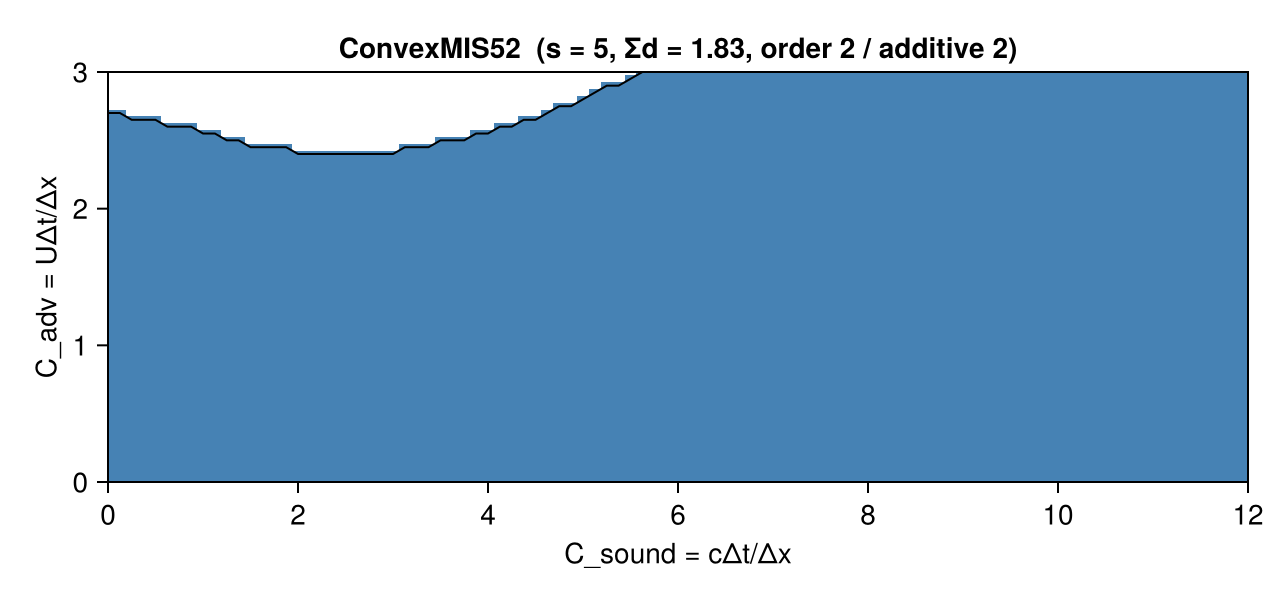
\includegraphics[width=0.8\textwidth]{stability_fv/ConvexMIS52.png}

\small\begin{tabular}{lcccccccc}\toprule $C_{\rm sound}$ & 0 & 2 & 4 & 8 & 12 & 16 & 20 & 24\\\midrule largest $C_{\rm adv}$ & 2.70 & 2.40 & 2.55 & 3.95 & 4.00 & 4.00 & 4.00 & 4.00\\\bottomrule\end{tabular}\end{center}
\noindent On the line $U/c=1/6$ stable up to $C_{\rm sound}\ge24.00$ ($C_{\rm adv}\ge4.00$). Base Runge--Kutta method, all explicit: $C_{\rm adv}\le2.70$ at $C_{\rm sound}=0$, $C_{\rm sound}\le0.750$ at $C_{\rm adv}=0$.
\clearpage
\section{ConvexMIS52r20}
Breeze.jl (branch \texttt{glw/mis-tableau-search}): as ConvexMIS52 with Shu--Osher coefficient 2.0.

\noindent $s=5$, $\Sigma d=1.6714$, orders G/B/A/L: 2 / 2 / 2 / 2.\\ Stage times $c=(0.4861, 0.4773, 0.6304, 0.9373, 1.0000)$.

{\footnotesize\[(\alpha_{ij})_{i\ge2}=\left(\begin{array}{rrrr}0.0479881465 &  &  & \\
0.1336999398 & 0.5372138662 &  & \\
0.3493364188 & 0.3121133954 & 0.1996477870 & \\
0.1497903665 & 0.2454583849 & 0.4340523780 & 0.0389024216\end{array}\right)\]
\[\beta=\left(\begin{array}{rrrrr}0.4861122626 &  &  &  & \\
0.0025905962 & 0.2399324874 &  &  & \\
0.0043468748 & 0.0021636972 & 0.3142110667 &  & \\
0.0037052042 & 0.0300090855 & 0.0023610807 & 0.3351315366 & \\
0.0003225063 & 0.0027917653 & 0.0021270072 & 0.0012672479 & 0.2442800933\end{array}\right)\]
\[(\gamma_{ij})_{i\ge2}=\left(\begin{array}{rrrr}0.4348918611 &  &  & \\
-0.1183228650 & 0.0960640555 &  & \\
-0.1198370411 & -0.2523734158 & 0.4761364842 & \\
-0.0360450529 & -0.1516682693 & -0.1355224350 & 0.4528769051\end{array}\right)\]}

\noindent Base Runge--Kutta method (\texttt{base\_method}; $F$ independent of its second argument), classical order 2:
{\footnotesize\[\begin{array}{r|rrrrr}0 &  &  &  &  & \\
0.4861122626 & 0.4861122626 &  &  &  & \\
0.4772569766 & 0.2373244892 & 0.2399324874 &  &  & \\
0.6304329296 & 0.1621142188 & 0.1541076442 & 0.3142110667 &  & \\
0.9373173487 & 0.2389996653 & 0.1484861694 & 0.2146999774 & 0.3351315366 & \\\hline
 & 0.2438052324 & 0.1443232356 & 0.2015134294 & 0.1660780093 & 0.2442800933\end{array}\]}

\begin{center}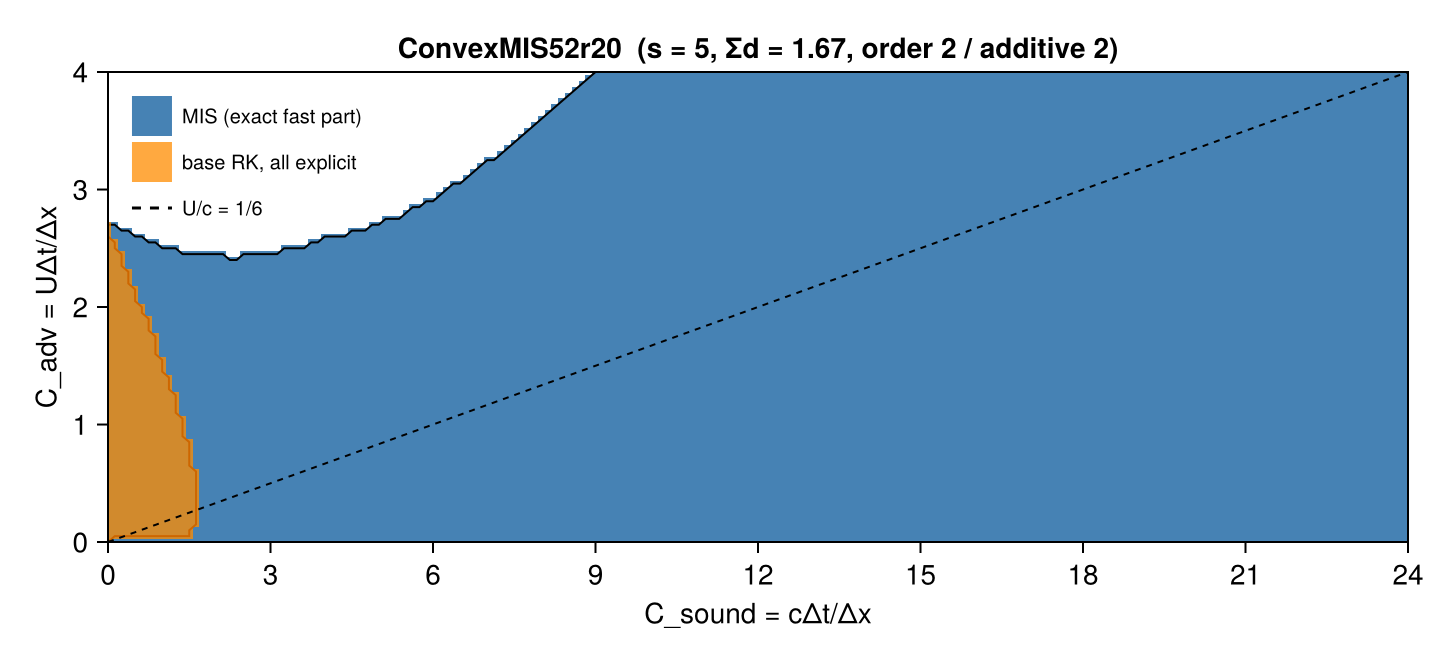
\includegraphics[width=0.8\textwidth]{stability_fv/ConvexMIS52r20.png}

\small\begin{tabular}{lcccccccc}\toprule $C_{\rm sound}$ & 0 & 2 & 4 & 8 & 12 & 16 & 20 & 24\\\midrule largest $C_{\rm adv}$ & 2.70 & 2.45 & 2.60 & 3.60 & 4.00 & 4.00 & 4.00 & 4.00\\\bottomrule\end{tabular}\end{center}
\noindent On the line $U/c=1/6$ stable up to $C_{\rm sound}\ge24.00$ ($C_{\rm adv}\ge4.00$). Base Runge--Kutta method, all explicit: $C_{\rm adv}\le2.70$ at $C_{\rm sound}=0$, $C_{\rm sound}\le0.000$ at $C_{\rm adv}=0$.
\clearpage
\section{ConvexMIS42}
Breeze.jl (branch \texttt{glw/mis-tableau-search}): 4 stages, as ConvexMIS52 (Shu--Osher coefficient 1.5).

\noindent $s=4$, $\Sigma d=1.6410$, orders G/B/A/L: 2 / 2 / 2 / 2.\\ Stage times $c=(0.5787, 0.6199, 0.8724, 1.0000)$.

{\footnotesize\[(\alpha_{ij})_{i\ge2}=\left(\begin{array}{rrr}0.0071760874 &  & \\
0.3042274603 & 0.4613122626 & \\
0.3301742627 & 0.3386730509 & 0.1315835193\end{array}\right)\]
\[\beta=\left(\begin{array}{rrrr}0.5786939080 &  &  & \\
0.0051603819 & 0.3285602874 &  & \\
0.0018549407 & 0.0016866408 & 0.4386866481 & \\
0.0011885024 & 0.0016901415 & 0.0013995714 & 0.2821114335\end{array}\right)\]
\[(\gamma_{ij})_{i\ge2}=\left(\begin{array}{rrr}0.4873295596 &  & \\
-0.2687812139 & 0.1995507165 & \\
-0.2032159415 & 0.0955885156 & 0.2936182195\end{array}\right)\]}

\noindent Base Runge--Kutta method (\texttt{base\_method}; $F$ independent of its second argument), classical order 2:
{\footnotesize\[\begin{array}{r|rrrr}0 &  &  &  & \\
0.5786939080 & 0.5786939080 &  &  & \\
0.6198880747 & 0.2913277873 & 0.3285602874 &  & \\
0.8724018362 & 0.2148952170 & 0.2188199712 & 0.4386866481 & \\\hline
 & 0.2925447907 & 0.2374138788 & 0.1879298970 & 0.2821114335\end{array}\]}

\begin{center}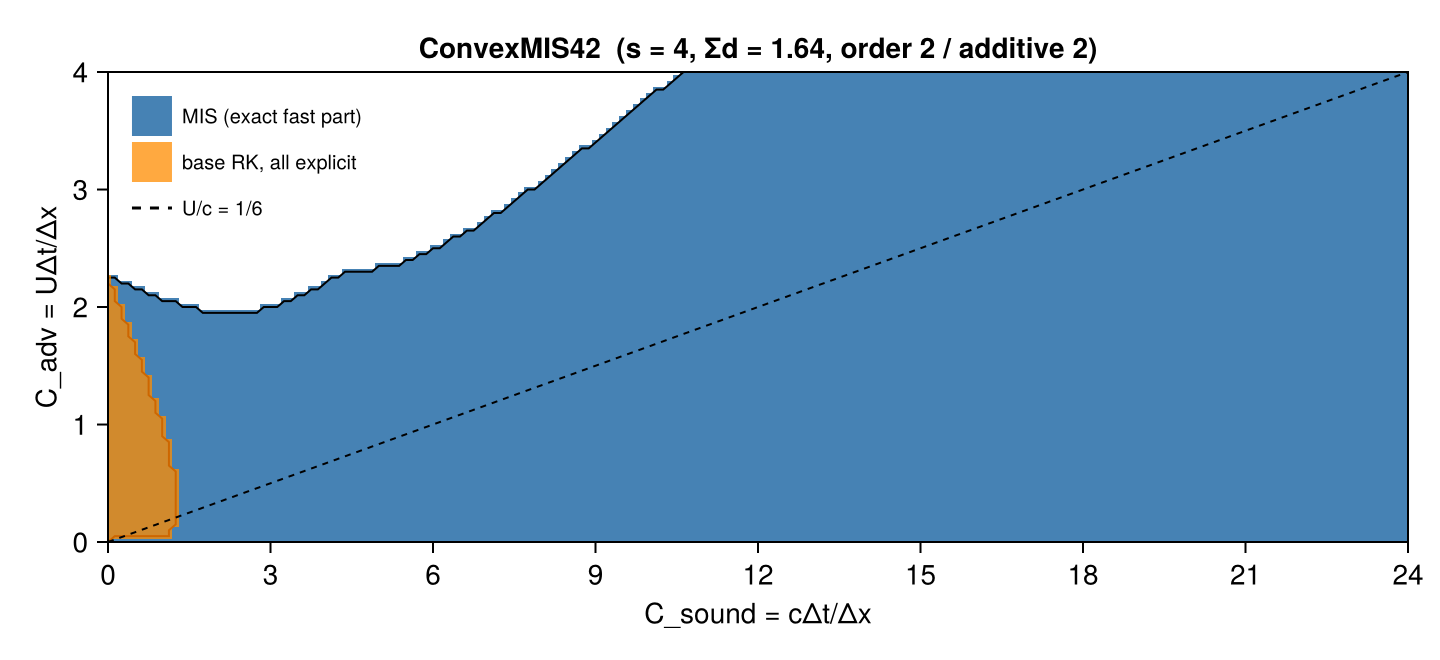
\includegraphics[width=0.8\textwidth]{stability_fv/ConvexMIS42.png}

\small\begin{tabular}{lcccccccc}\toprule $C_{\rm sound}$ & 0 & 2 & 4 & 8 & 12 & 16 & 20 & 24\\\midrule largest $C_{\rm adv}$ & 2.25 & 1.95 & 2.20 & 3.05 & 4.00 & 4.00 & 4.00 & 4.00\\\bottomrule\end{tabular}\end{center}
\noindent On the line $U/c=1/6$ stable up to $C_{\rm sound}\ge24.00$ ($C_{\rm adv}\ge4.00$). Base Runge--Kutta method, all explicit: $C_{\rm adv}\le2.25$ at $C_{\rm sound}=0$, $C_{\rm sound}\le0.000$ at $C_{\rm adv}=0$.
\end{document}
